
%\subsubsection{Process of AGG from Na2012 \cite{Na2012b} }
%TODO Edit in own words


Magnetostrictive Fe–Ga alloys (Galfenol) have promising attributes for application to sensors, actuators and energy harvesting as Clark et al. first reported in 2000\cite{clark2000magnetostrictive}. Single-crystal Galfenol has a body-centered
cubic (bcc) crystal structure, and along the \hkl<100> crystal orientations, it exhibits saturation magnetostriction of $\sim$400 ppm in low applied magnetic fields of $\sim$200 Oe. It also has a mechanical strength of $\sim$500 MPa, which is high relative to more costly rare earth magnetostrictive materials such as Terfenol-D alloys which exhibit giant magnetostriction ($\gtrsim$1600 ppm) but are brittle and require much higher magnetic fields ($\gtrsim$1000 Oe) for saturation\cite{clark2000magnetostrictive,Clark2003,Guruswamy2000}. The large magnetostriction and easy magnetization in single-crystal Galfenol alloys occur along the \hkl<100> orientation. It is thus desirable to obtain the \hkl<100> orientation in textured polycrystalline Galfenol, with the goal of providing enhanced mechanical properties and lower cost than single-crystal material, with similar magnetostrictive strain. 

Two viable approaches have been employed to fabricate highly textured Fe–Ga alloys\cite{srisukhumbowornchai2001large,kellogg2003texture}. One is a directional solidification growth process, and the other is thermomechanical processing involving deformation via rolling and recrystallization through grain growth and orientation mechanisms. Galfenol rods grown by the directional solidification process have strong crystallite textures with \hkl<100> preferred orientation aligned 14$^{\circ}$ off from the rod direction and a maximum magnetostriction ($\lambda_{\parallel}$) of 271 ppm under compression \cite{srisukhumbowornchai2001large}. In other works, Kellogg et al. reported that binary Fe$_{0.83}$Ga$_{0.17}$ with a somewhat dispersed \hkl{001}\hkl<100> texture along rolling direction (RD) exhibited magnetostrictive strain of $\sim$160 ppm as a consequence of rolling and annealing at 1100$^{\circ}$C for 4 h\cite{kellogg2003texture}. Texture annealing of Fe$_{0.85}$Ga$_{0.15}$ alloy with 1 mol.\% NbC at 1150–1300$^{\circ}$C for 24 h changed the texture from a strong $\alpha$-fiber texture \hkl<110>$\parallel$RD in as-rolled sheet to a preferred texture with \hkl<100> orientation\cite{srisukhumbowornchai2004crystallographic}. The authors did not report the magnetostriction values; however, an estimated of lower than 135 ppm can be made based on their electron backscatter diffraction (EBSD) data and the nominal saturation value in a single crystal with the same composition. In our prior work, we have demonstrated the texture development of Goss \hkl{011}\hkl<100> texture through secondary recrystallization by using NbC particles as an inhibitor of normal grain growth(NGG) \cite{Na2009}.

%TODO: Connect AGG to surface energy

\subsubsection{Need for Surface Energy}

\textbf{Galfenol} 
%\textbf{Galfenol AGG is affected by sulfur surface segregation concentration}

We have been studying the development of Goss- and Cube-textured Galfenol rolled sheet as a low-cost alternative to magnetostrictive single crystal Galfenol for several years. We targeted Goss and Cube textures to obtain one and two directions respectively of easy magnetic axes and high magnetostriction in the plane of the rolled sheet. An additional benefit of developing a Cube texture is that it will make feasible use magnetic field annealing to maximize performance\cite{Yoo2008,Yoo2009} and thereby eliminate the need for stress annealing or use of prestress components in the design of devices that use these materials.\cite{Restorff2006,Summers2009b} Developing protocols for making thin sheet Galfenol with Goss or Cube textures has been challenging because the mechanisms that regulate grain boundary mobility and texture development in these alloys are not well understood. The preliminary results in Fig. \ref{fig:AGG-diagram} show AGG and texture development in Galfenol rolled sheet for several different anneal protocols. The dramatic difference in AGG and texture between the result in the top right image and the results in the two lower right images was accomplished by building on empirical insights from studies of Fe and Fe-Si alloys in which control of surface energy was used to regulate grain growth and ultimately to produce Cube-textured material.\cite{Walter1965,dunn1962surface,waeckerle1993effect,Kramer1992}

\begin{figure}[h!] 
	\centering
	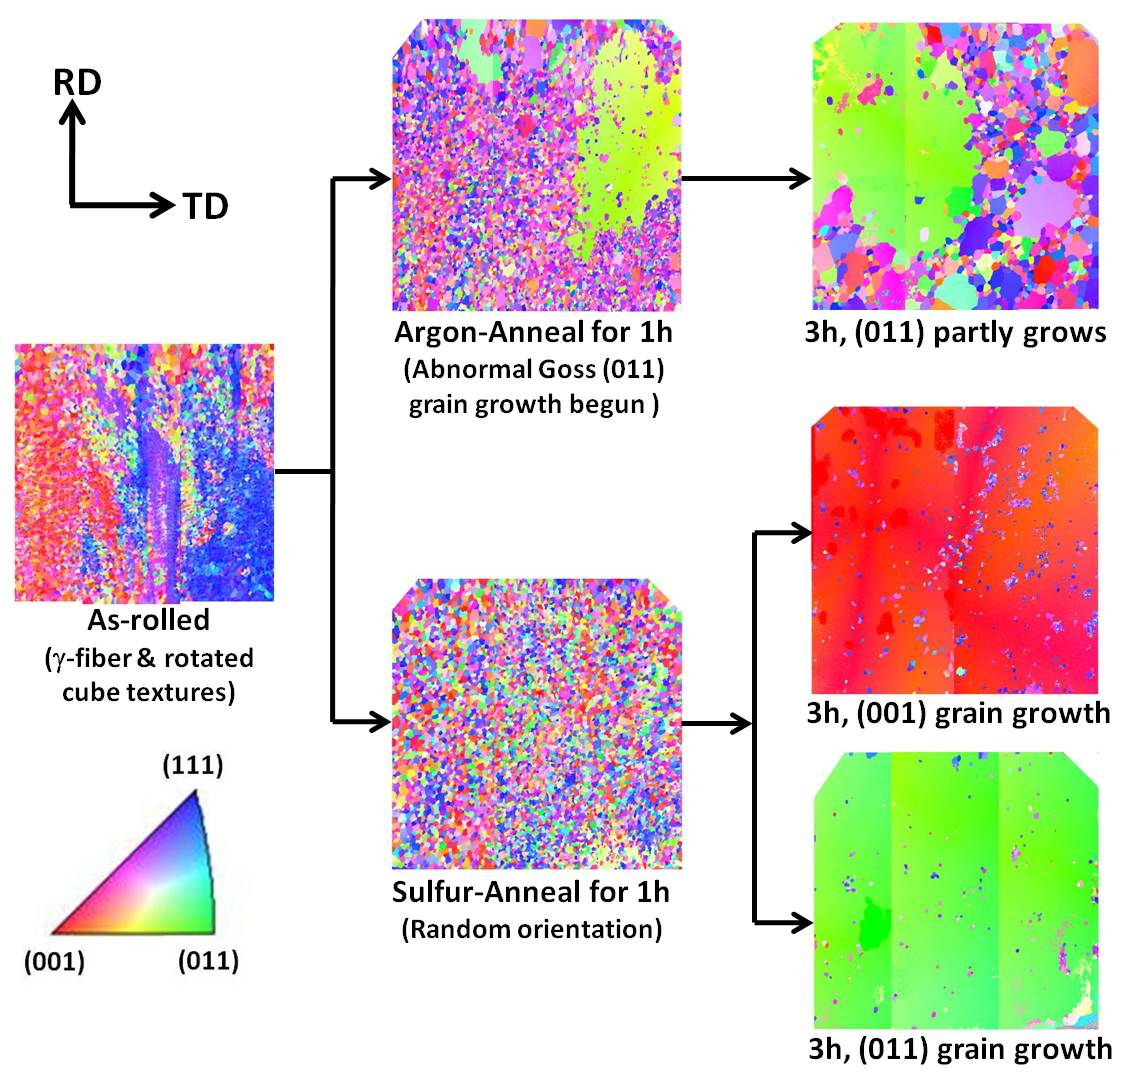
\includegraphics[width=0.6\textwidth]{AGG-diagram}
	\caption{Diagram of AGG from as-rolled sample of (Fe-19$\%$Ga)+1.0$\%$NbC alloy (left) to argon- (upper) and sulfur-annealed (lower) samples for annealing times of 1h (middle) and 3h (right). EBSD images scanned along the normal direction of 12x12x0.45 mm$^{3}$ sheet. Red, green and blue indicate \hkl(001), \hkl(011) and \hkl(111) grains, respectively. 
	}
	\label{fig:AGG-diagram}		
\end{figure}

In Fig. \ref{fig:AGG-diagram}, as-rolled polycrystalline Galfenol (left image) exhibits a strong $\gamma$-fiber and weak rotated cube textures, and starts with an $\alpha$-iron (B2) structure. A partly grown Goss texture developed over $\sim$39$\%$ of the sample surface area during a 3h argon-anneal (upper right image) due to grain boundary energy alone. We have also demonstrated that small variations in surface energy have a significant impact of the development of texture.\cite{Chun2010,Na2012b} The two lower right images show AGG with fully developed \hkl(001) and \hkl(011) grains over 90-95$ \% $ of the sample surface. AGG of (011) grains is very reproducible (insensitive to small variations in anneal conditions), while the development of (001) grains is challenging to produce/reproduce (highly sensitive to anneal conditions). Saturation magnetostriction values equal to 90$ \% $ and 84$ \% $ of single crystal \hkl(100) values for alloy of the same composition were measured in sulfur-annealed samples with \hkl(001) and \hkl(011) grain growth, respectively. Auxeticity of these samples has not been investigated. 


Figure \ref{fig:AGG-diagram} results are the first and only that we know of to employ concepts that date back to the mid-1960’s \cite{Walter1965,dunn1962surface,waeckerle1993effect} for developing AGG in irons, Fe-Si and silicon-steels together with Kramer’s work in the 1990’s\cite{Kramer1992} on control of surface energy to develop Cube texture in Fe-Si. Our research hypothesis is motivated by our desire to understand the physical metallurgy that lead to these results and be able to routinely reproduce these results in rare-earth-free anisotropic alloys. \\
\textbf{Alfenol}

The importance of Alfenol surface energy lies in the Aerosmart Lab's need for more efficient energy harvesting materials, as discussed in Section \ref{magnetostrict-materials}. Currently, stress-annealed and field-annealed samples are first rolled into sheets from ingots, and then atmospherically annealed to develop large grains that cover over 90\% of the sample surface area. This process avoids lengthy and expensive single-crystal growth methods. We target Goss \hkl{110} and Cube \hkl{100} textures to obtain one and two directions, respectively, of easy magnetic axes and high magnetostriction in the plane of the rolled sheet. Goss-textured Alfenol can reach magnetostrictive constants of ~184 ppm, and the elusive Cube-textured Alfenol would reach even higher magnetostriction values due to the additional direction of easy magnetic axes. An added benefit of developing a Cube texture is that it will make feasible use of magnetic field annealing to maximize performance\cite{Yoo2009,Yoo2008} and thereby eliminate the need for stress annealing or use of pre-stress components in the design of devices that use these materials\cite{Restorff2006,Summers2009}. Clearly, Alfenol AGG is affected differently than Galfenol under sulfur concentrations. This must be due to the differences in orientation-dependent surface energy between Galfenol and Alfenol.
	
